\documentclass[12pt,letterpaper]{article}
\usepackage{natbib}

%Packages
\usepackage{pdflscape}
\usepackage{fixltx2e}
\usepackage{textcomp}
\usepackage{fullpage}
\usepackage{float}
\usepackage{latexsym}
\usepackage{url}
\usepackage{epsfig}
\usepackage{graphicx}
\usepackage{amssymb}
\usepackage{amsmath}
\usepackage{bm}
\usepackage{array}
\usepackage[version=3]{mhchem}
\usepackage{ifthen}
\usepackage{caption}
\usepackage{hyperref}
\usepackage{amsthm}
\usepackage{amstext}
\usepackage{enumerate}
\usepackage[osf]{mathpazo}
\usepackage{dcolumn}
\usepackage{lineno}
\usepackage{dcolumn}
\newcolumntype{d}[1]{D{.}{.}{#1}}

\pagenumbering{arabic}


%Pagination style and stuff
\linespread{2}
\raggedright
\setlength{\parindent}{0.5in}
\setcounter{secnumdepth}{0} 
\renewcommand{\section}[1]{%
\bigskip
\begin{center}
\begin{Large}
\normalfont\scshape #1
\medskip
\end{Large}
\end{center}}
\renewcommand{\subsection}[1]{%
\bigskip
\begin{center}
\begin{large}
\normalfont\itshape #1
\end{large}
\end{center}}
\renewcommand{\subsubsection}[1]{%
\vspace{2ex}
\noindent
\textit{#1.}---}
\renewcommand{\tableofcontents}{}
%\bibpunct{(}{)}{;}{a}{}{,}

%---------------------------------------------
%
%       START
%
%---------------------------------------------

\begin{document}

%Running head
\begin{flushright}
Version dated: \today
\end{flushright}
\bigskip
\noindent RH: Branch swapping algorithm

\bigskip
\medskip
\begin{center}

\noindent{\Large \bf SPR/TBR.} %TG: Need a title!
\bigskip

\noindent {\normalsize \sc Thomas Guillerme$^1$$^*$, and Martin D. Brazeau$^1$}\\ %TG: Author order can be swapped of course! There's only a finite combination of 2 elements anyway!
\noindent {\small \it 
$^1$Imperial College London, Silwood Park Campus, Department of Life Sciences, Buckhurst Road, Ascot SL5 7PY, United Kingdom.\\}
\end{center}
\medskip
\noindent{*\bf Corresponding author.} \textit{t.guillerme@imperial.ac.uk}\\  %TG: Same as above
\vspace{1in}

%Line numbering
\modulolinenumbers[1]
\linenumbers

%---------------------------------------------
%
%       ABSTRACT
%
%---------------------------------------------

\newpage
\begin{abstract}
blablabla
\end{abstract}

\noindent (Keywords: )\\

\vspace{1.5in}

\newpage 

%---------------------------------------------
%
%       INTRODUCTION
%
%---------------------------------------------

\section{Introduction}

Tree rearrangement is used in phylogenetic inference or in macroecology and macroevolution (e.g. comparing trees) %TG: Potential selfcite here!
+ linguistic and philology
-linguistic tree searching, but that's really phylogenetics. Linear model simplification has parallels too.
-similar to search strategies in integer and mixed integer programming - it's all combinatorial optimisation.
But also used in network analysis?
Or horizontal genes transfer analysis? \citep{mcfadden1995something}.
If two trees of two different sets of genes for the same species have a different topology, and that the inconsistency can be resolved by a single hybridisation event, there is a single subtree pruning regrafting (SPR) operation that can solve the problem \citep{bordewich2005computational}.



Classic literature will visit redundant trees \citep{felsenstein2004inferring}.

That takes time and introduces statistical biases (e.g. for heuristic searches, some topologies can be visited more than others).
This can be problematic. For example, for a tree with $n$ taxa, SPR/TBR can produce $M$ topologies including $m$ similar ones.
If the tree search algorithm is set to subsample $m$ topologies only, it has a possibility to subsample the $m$ similar topologies only thus being literally ineffective at exploring tree space.


Therefore it's important to implement branch swapping algorithms properly.

Here we propose a method that is equivalent mathematically to the previous ones \citep{felsenstein2004inferring} but that uses a different practical approach that can be more intuitive and allows to visit each topology only once.

We look at SPR as rerooting + branching.

Number of rooted binary trees for $n$ taxa:
\begin{equation}
(2n-3)!!=(2n-3)\times(2n-5)\times...\times3=\frac{(2n-2)!}{2^{n-1}(n-1)!}
\end{equation}

\section{NNI, SPR and TBR}

\subsection{Tree elements definition}
\begin{itemize}
    \item a \textbf{tip} is any leaf of the tree (degree 1 vertices) that is connected to only one node.
    \item a \textbf{node} is formed by the connection of tips or nodes. In a binary tree, a node has exactly one ancestor (or parent) and two descendants.
    \item an \textbf{edge} is any single connection between two nodes or a node and a tip.
    \item the \textbf{root} is the single edge that is only connected to one node (and nothing).
\end{itemize}

Probably reuse the figure from Felsenstein modified. %TG: or from wiki?

Definitions: \cite{allen2001subtree,felsenstein2004inferring}


\begin{figure}[!htbp]
\centering
   \includegraphics[width=0.8\textwidth]{Figure/FelsensteinFigure.pdf}
\caption{\scriptsize{SPR and TBR description. Modified from \cite{felsenstein2004inferring}, Figure 4.5 and 4.6. \textbf{SPR-1:} blabla; \textbf{SPR-2:} blabla; \textbf{SPR-3:}blabla; \textbf{TBR-1:} blabla; \textbf{TBR-2:} blabla (note that when the sub-tree is reroot on position \textit{1}, the rearrangement is equivalent to a SPR); \textbf{TBR-3:}blabla.}}
\label{Figure_Felsenstein}
\end{figure}


\section{Improved algorithm}

\subsection{Neighbour Rule}
Neighbour Rule described \citep[in other words;][]{allen2001subtree}.

\subsection{SPR as TRB (Subtree Rerooting and Branching)}

\section{Conclusion}

This way is not different than the classic SPR/TBR but it's a better implementation.

\section{Data availability and reproducibility}
%TG: Probably some link to morphy


\section{Acknowledgments}
European Research Council under the European Union’s Seventh Framework Programme (FP/2007–2013)/ERC Grant Agreement number 311092.


\bibliographystyle{sysbio}
\bibliography{References}

\end{document}
